\documentclass[a4paper,12pt]{article} %style de document
\usepackage[utf8]{inputenc} %encodage des caractères
\usepackage[french]{babel} %paquet de langue français
\usepackage[T1]{fontenc} %encodage de la police
\usepackage[top=2cm,bottom=2cm,left=2cm,right=2cm]{geometry} %marges
\usepackage{graphicx} %affichage des images
\usepackage{amssymb}
\usepackage{url}
\usepackage{verbatim}
\usepackage{amsmath}
\usepackage{tikz}
\usepackage{hyperref}
\hypersetup{
	hidelinks,
    colorlinks,
    citecolor=black,
    filecolor=black,
    linkcolor=black,
    urlcolor=black
}

\begin{document} %début du document

%----------------------------------
%page de garde
%----------------------------------

\begin{titlepage}

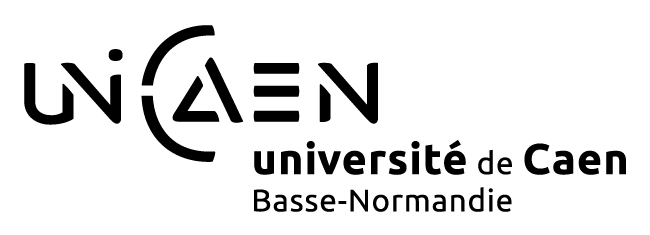
\includegraphics[scale=0.3]{images/unicaen.png}

\vspace{7cm}

\begin{center}

\begin{Huge}
TPA\\
Rapport de Projet\\
\end{Huge}
\vspace{2cm}
\begin{large}
Beauchamp Aymeric 21301016\\
Chagneux Dimitri 21606807\\
Mori Baptiste 21602052\\
Leblond Valentin 21609038\\
\vspace{1cm}
L2-Info-groupe-4A
\end{large}

\end{center}
\end{titlepage}


%------------------------------
%sommaire
%------------------------------

\newpage

\tableofcontents

\newpage

%------------------------------
%contenu
%------------------------------


\section*{Objectifs}
\addcontentsline{toc}{section}{Objectifs}

\subsection*{Description du Sokoban}
\addcontentsline{toc}{subsection}{Description du Sokoban}

Le Sokoban est un jeu de réflexion de type puzzle où le joueur doit placer des caisses sur des objectifs placés à l'avance sur la carte. Le joueur gagne si toutes les caisses sont placées sur les objectifs et il ne peut pousser qu'une seule caisse à la fois. Il existe de nombreux niveaux dont la difficulté est variable.

\begin{figure}[!h]
\centering
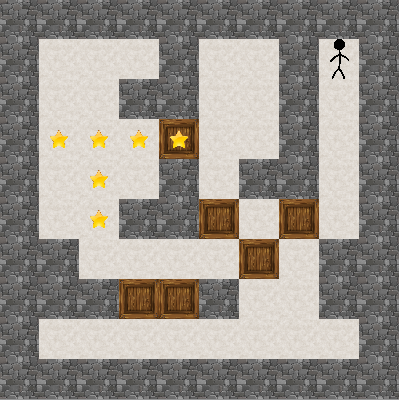
\includegraphics[scale=0.5]{images/sokoban.png}
\caption{Niveau de Sokoban}
\end{figure}

\subsection*{Les fonctionnalités attendues}
\addcontentsline{toc}{subsection}{Les fonctionnalités attendues}

Pour ce projet, nous devions mettre au point une version jouable pour un humain en console, en prenant en compte l'importation de niveaux (au format \textbf{.xsb}). Il était également demandé de réaliser une interface graphique et une fonctionnalité permettant une résolution automatique de niveau.\\
Enfin, permettre de faire jouer en parallèle un humain et un ordinateur, et rendre \textit{anytime} l'algorithme de l'intelligence artificielle. C'est à dire le fait que lorsque le joueur fait un mouvement, l'intelligence artificielle doit en faire un.


\section{Fonctionnalités implémentées}

\subsection{Description des fonctionnalités}

\subsubsection*{Attendues}
\addcontentsline{toc}{subsubsection}{Attendues}

La version console fonctionne à l'aide de saisies de l'utilisateur qui lui permettent de contrôler le jeu. Une fois un niveau terminé, on demande au joueur si il souhaite passer au niveau suivant.\\

La carte est chargée à partir d'un fichier \textbf{.xsb} contenant des lignes de caractères, que l'on transforment en liste de caractères.\\
La carte est donc modélisée par des chaînes de caractères:
\begin{itemize}
\item \textbf{\#} pour un mur
\item \textbf{\$} pour une caisse
\item \textbf{@} pour le joueur
\item \textbf{.} pour un objectif
\item \textbf{*} pour une caisse sur un objectif
\item \textbf{+} pour le joueur sur un objectif
\item \textbf{espace} pour les cases vides
\end{itemize}

\begin{figure}[!h]
\centering
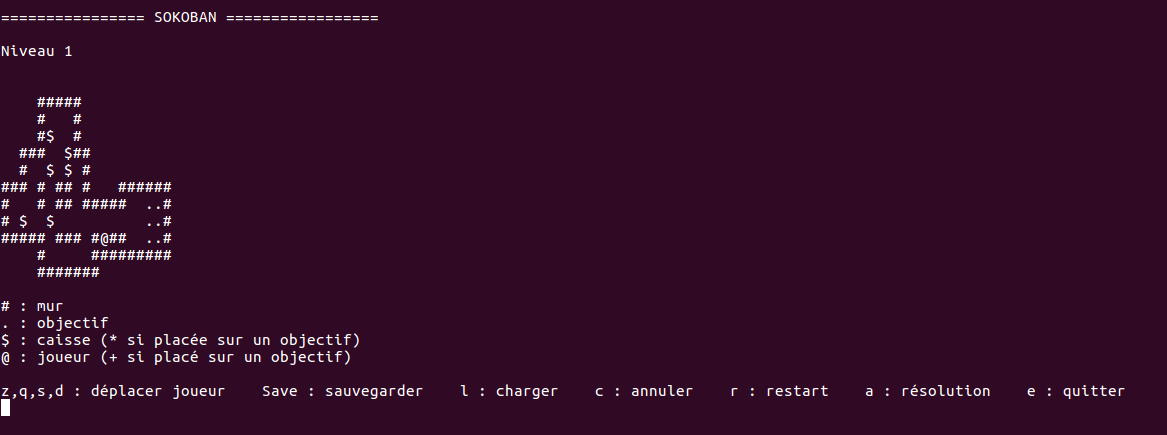
\includegraphics[scale=0.5]{images/Capture.png}
\caption{Interface console}
\end{figure}

Au niveau de l'interface graphique, nous avons une zone de jeu dans laquelle on dessine le niveau et des boutons pour gérer les différentes fonctionnalités. Le personnage est déplaçable avec les flèches directionnelles ou ZQSD, si le joueur a bloqué une caisse ou si il a gagné, il ne peut plus bouger et doit recommencer le niveau ou passer au suivant (seulement si il a gagné). Si le joueur gagne, le personnage effectue le Dab et si il perd, le personnage pleure.\\

Il est possible de demander la résolution automatique du niveau. Un solveur calcule alors un itinéraire permettant de ranger toutes les caisses à partir de la position du joueur.

\begin{figure}[!h]
\centering
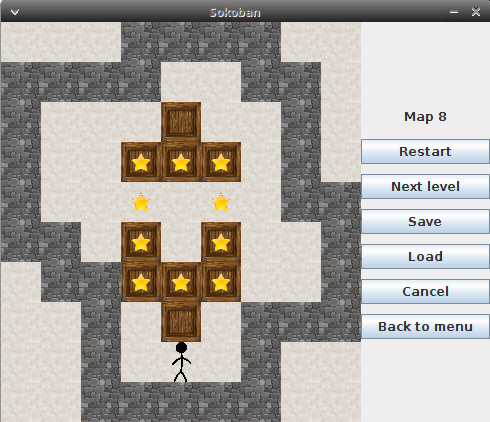
\includegraphics[scale=0.5]{images/Capture2.png}
\caption{Interface graphique}
\end{figure}

\subsubsection*{Ajoutées}
\addcontentsline{toc}{subsubsection}{Ajoutées}

Au lancement du programme, l'utilisateur peut choisir un profil ou en créer un nouveau.\\
En fonction de l'avancement du profil donné, le joueur a débloqué un certain nombre de cartes ; pour débloquer la carte suivante il faut finir le niveau en cours. Lorsqu'un profil est chargé, la dernière carte non terminée est lancée automatiquement.\\

Nous proposons également à l'utilisateur de sauvegarder sa partie à un instant du niveau donné, de charger sa sauvegarde (il n'y a pas de conflit entre les sauvegardes des différents utilisateurs), d'annuler le dernier coup joué  et enfin de recommencer le niveau courant.

\subsection{Organisation du projet}

Pour le début du projet, nous avons tous travaillé sur la conception du modèle du jeu : comment représenter chaque élément qui compose le jeu (joueur, case vide, caisse ou encore la carte qui les contiendra). Ensuite nous nous sommes interrogés sur la manière de déplacer le joueur ainsi que faire pousser les caisses par le joueur et faire en sorte de gérer les collisions avec les murs.\\
Nous avons rencontrés des difficultés pour la détection d'une caisse bloquée. Nous nous sommes d'abord contentés de considérer le cas où une caisse est bloquée par deux murs de telle façon qu'il est impossible de la déplacer (cas de gauche de la \textbf{figure \ref{figure4}}).\\
Nous nous sommes vite rendus compte que ce n'était pas le seul cas de caisse bloquée, comme on peut le voir sur la deuxième image de la \textbf{figure \ref{figure4}}. En effet, on ne peut déplacer aucune des deux caisses car elles se bloquent entre elles. Nous avons donc gérer ce cas, mais il était loin d'être le dernier, le sokoban étant un jeu très facile à bloquer. Les cas plus complexes sont traités dans la partie \hyperref[et]{Eléments techniques}.

\begin{figure}[!h]
\centering
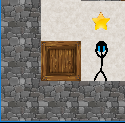
\includegraphics[scale=0.5]{images/Capture3.PNG}
\hspace{1cm}
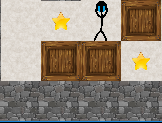
\includegraphics[scale=0.5]{images/Capture4.PNG}
\caption{Blocage simple de caisses}
\label{figure4}
\end{figure}

Ensuite, nous nous sommes séparés en trois groupes, deux d'entre nous ont débuté la conception d'une IA capable de résoudre des niveaux du jeu, et une autre personne s'est lancée dans la création de la classe principale avec interface console ainsi que toute la gestion de fichiers (sauvegarde, chargement, traduction entre une carte enregistrée dans un fichier et notre représentation d'un niveau de notre code). Le dernier membre s'est occupé de gérer les cas complexes de détections de caisses bloquées puis s'est attelé au développement de l'interface graphique.\\

L'interface graphique ayant bien avancé, des nouvelles fonctionnalités ont été ajoutées dans celle-ci (telles que la sélection de profils) et des réglages dans la manière de sauvegarder une map ont été modifiés, ce qui a posé problème : le modèle était devenu obsolète par rapport à l'interface graphique. Il a donc fallu revoir notre classe principale pour y implémenter la gestion de profils, et changer la manière de sauvegarder une map car la première version ne nous permettait pas de recommencer le niveau courant.\\

Au niveau de l'IA, nous avons d'abord conçu un système de déplacement automatique du joueur avant de concevoir un solveur. Nous avons passé beaucoup de temps sur une première implémentation techniquement fonctionnelle mais incapable de résoudre des niveaux qui ne soient pas extrêmement simples, avant de passer à une seconde implémentation bien plus efficace et utilisant les outils développés pour la première. 

\section{Éléments techniques}\label{et}

\subsection{Gestion des deadlocks}

\subsection{Structures de données utilisées}

Le niveau de sokoban, une fois lu dans un fichier .xsb, est représenté avec une grille d'objets. Le principal avantage de cette méthode est l'intuitivité de la représentation.
Les positions des caisses et des objectifs sont stockées dans des listes du fait de l'importance de ces informations. Cela évite de devoir charger la grille dès qu'on a besoin d'une position.\\

Dans le package ia, nous utilisons des tables de hashage avec les algorithmes de recherche en tant que mémoire. Cela nous permet de pouvoir vérifier rapidement si un élément a déjà été vu, surtout lorsque l'on explore plusieurs centaines de milliers d'états.
Le solveur lui-même tient sa performance d'une file de priorité qui guide la recherche de la solution.

\subsection{Algorithmes de l'IA}

\subsubsection{Déplacement du joueur}

Pour obtenir une granularité dans le déplacement du joueur par l'IA, nous avons implémenté l'algorithme de recherche de chemin A*. On utilise des objets \textbf{Node} qui possédent en attribut des coordonnées et un nœud prédécesseur. Pour chaque nœud, on calcul le coût du chemin entre le départ et la destination passant par ce nœud. Le coût du chemin s'exprime :

$$ f(x) = g(x) + h(x)$$

où $g(x)$ est le coût du chemin depuis le départ et $h(x)$ est une fonction heuristique estimant le coût pour atteindre la destination.\\

Le calcul de $g(x)$ consiste à compter récursivement les prédécesseurs du nœud jusqu'à arriver au départ.\\
L'heuristique utilisée pour $h(x)$ est la distance de Manhattan : la décomposition de la distance euclidienne entre deux points en une composante verticale et une composante horizontale. Cette heuristique est adaptée au Sokoban étant donné qu'on ne peut pas se déplacer en diagonale. Elle est également admissible pour A* : elle ne sous-estime jamais la distance à l'arrivée. Cela garantit que le chemin trouvé est optimal.

\begin{figure}[!h]
\centering
\begin{tikzpicture}
\node (depart) at (0,0) {A};
\node (arrivee) at (2,2) {B};
\coordinate (x) at (2,0);
\draw[color=blue] (depart) -- node[left] {Distance euclidienne}(arrivee);
\draw[color=red] (depart) -- node[below] {Distance de Manhattan} (x);
\draw[color=red] (x) -- (arrivee);
\end{tikzpicture}
\caption{Illustration de la distance de Manhattan}
\end{figure}

Le fonctionnement de cet algorithme est le suivant :\\

\begin{itemize}
\item On initialise l'algorithme avec les positions du joueur et de sa destination et on ajoute la position du joueur dans une liste d'attente. On crée aussi deux tables de hashage avec autant de clés qu'il y a de positions libres dans la grille. Les clés sont des objets Node ; à ces clés sont associées la valeur du nœud que l'on initialise à +$\infty$.
\item On retire de la liste d'attente l'élément ayant le plus faible $f(x)$ et on vérifie si il correspond à la destination. Si ce n'est pas le cas, on le met dans une liste des noeuds explorés.
\item On 
\end{itemize}
  
\begin{figure}[!h]
\centering
\begin{tikzpicture}
\node at (0,0) {@};
\draw (0,0) circle(0.5);
\node at (1,0) {2};
\draw (1,0) circle(0.5);
\node at (2,0) {4};
\draw (2,0) circle(0.5);
\node at (0,1) {1};
\draw (0,1) circle(0.5);
\node at (0,2) {3};
\draw (0,2) circle(0.5);
\node at (1,2) {5};
\draw (1,2) circle(0.5);
\node[draw=black] at (2,1) {\#};
\node at (2,2) {.};
\draw (2,2) circle(0.5);
\node at (3,0) {6};
\draw (3,0) circle(0.5);
\node at (3,1) {8};
\draw (3,1) circle(0.5);
\node at (3,2) {9};
\draw (3,2) circle(0.5);
\node[draw=black] at (1,1) {\#};
\draw[->, color=red] (0,0) -- (0,1);
\draw[->, color=red] (0,1) -- node[left] {chemin trouvé} (0,2);
\draw[->, color=red] (0,2) -- (1,2);
\draw[->, color=red] (1,2) -- (2,2);
\draw[->] (0,0) -- (1,0);
\draw[->] (1,0) -- node[below] {chemin exploré} (2,0);
\draw[->] (2,0) -- (3,0);
\end{tikzpicture}
\caption{Exemple d'exécution de A* pour le déplacement}
\end{figure}

\subsubsection{Solveurs}

\section{Architecture du projet}

\subsection{Organisation des packages}

Notre projet se décompose en trois packages distincts:
\begin{itemize}
\item le package \textbf{sokoban}, le package principal contenant le modèle du sokoban, et la gestion de fichier, utilisé dans les deux autres packages;
\item le package \textbf{graphique}, qui gère l'interface graphique;
\item le package \textbf{ia}, qui implémente les algorithmes de résolution automatique.
\end{itemize}

En créant ces trois packages, nous avons pu travailler en parallèle sur différents aspects du projet sans pour autant se gêner les uns les autres.
Ainsi, une modification du package \textbf{ia} ne changeait rien au fonctionnement du sokoban en version console ou graphique.\\
Cependant, après modification du package \textbf{sokoban}, tout le groupe devait récupérer la version la plus récente, car ce package est utilisé par les deux autres puisqu'il contient le modèle.

\begin{figure}[!h]
\centering
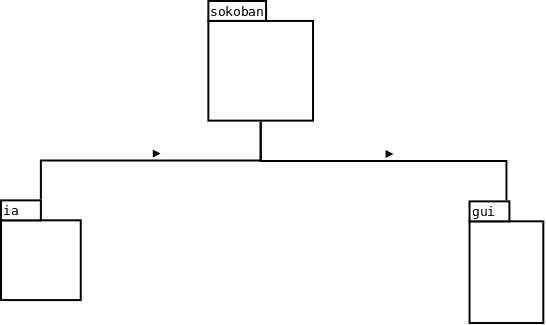
\includegraphics[scale=0.5]{images/packages.png}
\caption{Diagramme du projet}
\end{figure}

\subsection{Organisation des classes}

\subsubsection{Package sokoban}

Notre package principal comporte treize classes réparties en différentes catégories:
\begin{itemize}
\item les classes gérant les entités (personnage, murs, ...);
\item les classes permettant d'enregistrer/charger une sauvegarde;
\item les classes permettant de lancer le programme.
\end{itemize}

Toutes les classes de gestion des entités héritent de la classe \textit{Block}, elles permettent de déplacer facilement le personnage et les caisses, de gérer les collisions, les blocages et la fin d'une partie.

Les classes gérant les fichiers permettent de lire et d'écrire dans des fichiers situés dans un dossier "maps" contenant toutes les cartes du jeu, ou dans un fichier "save" stockant les profils et leur sauvegarde/cancel.

Les classes permettant de lancer le programme sont le Board, qui créer la grille de jeu, et le Main.

\begin{figure}[!h]
\centering
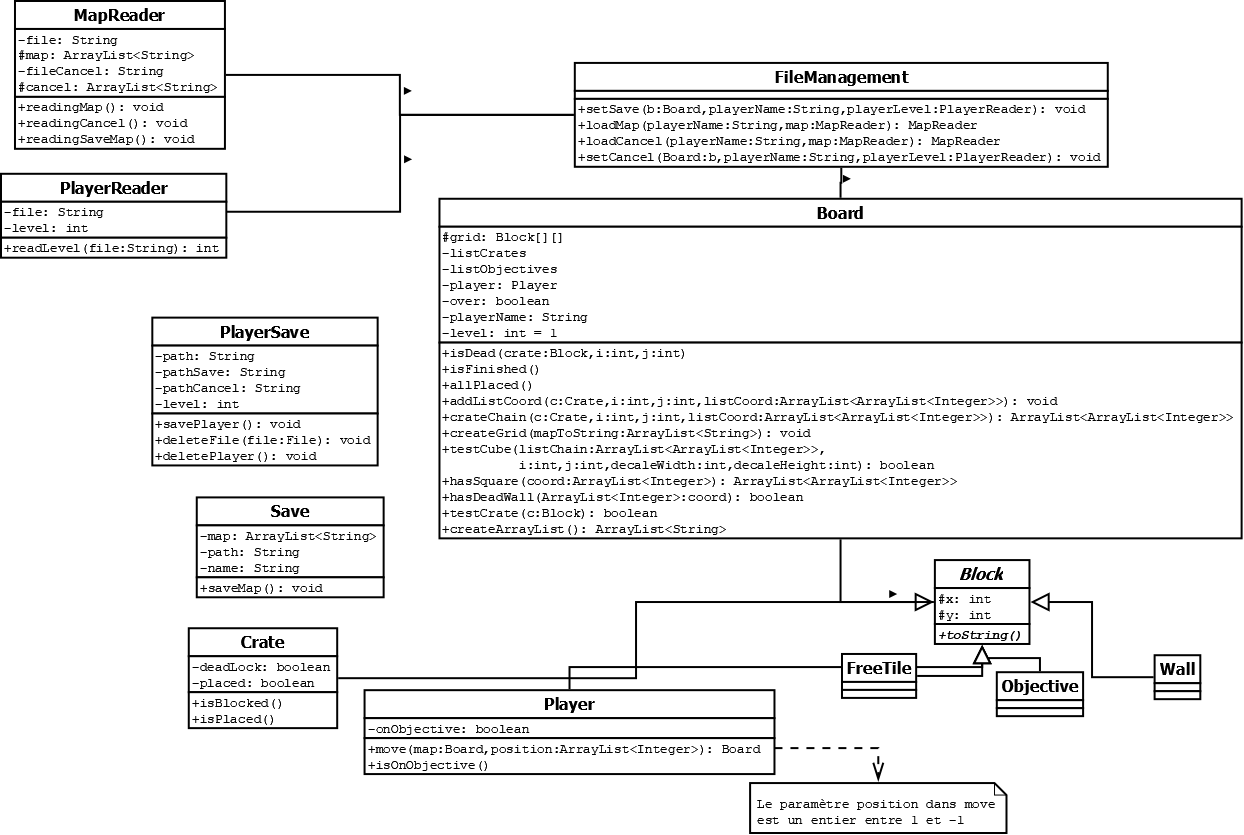
\includegraphics[scale=0.5]{images/diag_sokoban.png}
\caption{Diagramme du package sokoban}
\end{figure}

\subsubsection{Package graphique}

Ce package permet simplement de gérer la version graphique du Sokoban et de jouer sans les entrées claviers (en appuyant directement sur une touche, on peut déplacer le joueur).

\begin{figure}[!h]
\centering
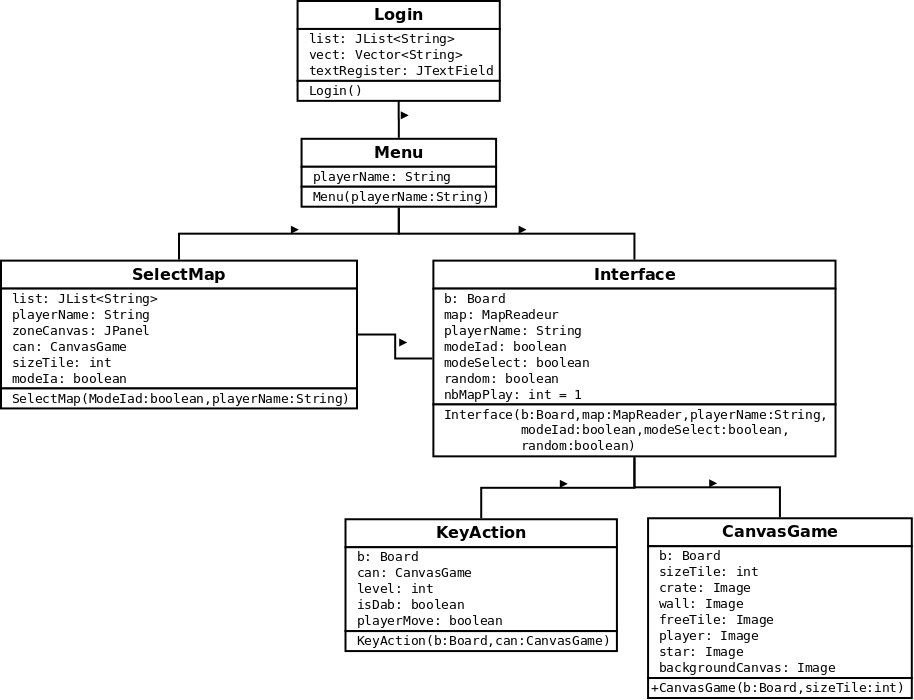
\includegraphics[scale=0.4]{images/graphique.png}
\caption{Diagramme du package graphique}
\end{figure}

\subsubsection{Package ia}

Ce package contient tout ce qui a trait à la résolution automatique du jeu. On y trouve des classes décrivant des concepts du jeu, 

\begin{figure}[!h]
\centering
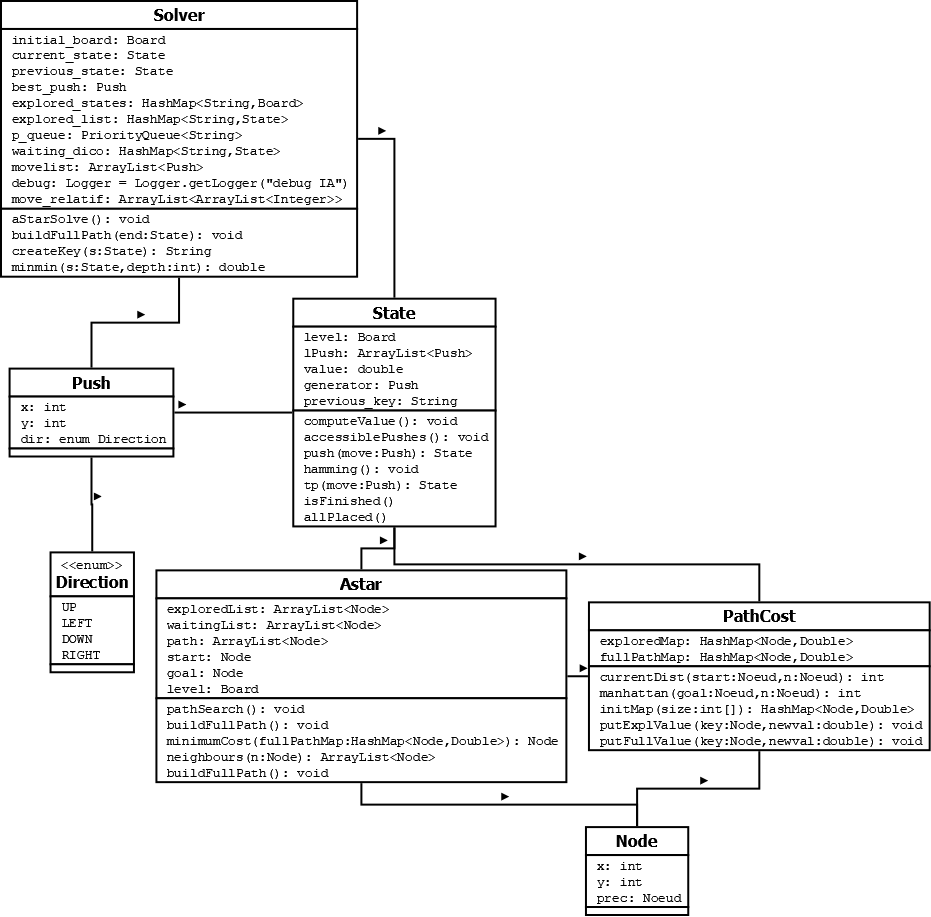
\includegraphics[scale=0.5]{images/diag_ia.png}
\caption{Diagramme du package ia}
\end{figure}

\section{Expérimentations et usages}

\subsection{Performance du solveur}

\section*{Conclusion}
\addcontentsline{toc}{section}{Conclusion}


\end{document}

